\chapter{Model based on Inertial Measurement Unit}
\label{chap:simp_mdl}
In this chapter a simplified dynamic model of motion equations is used in the prediction step of EKF. The model is based on the translational acceleration and angular velocity measured by IMU. The ODE's are formulated based on Equation \ref{eq:newton_motion}.

\section{Simplified motion model}
IMU \emph{MTi-100 \footnote{xsens technologies \url{http://www.xsens.com/en/general/mti-100-series} }} consists of accelerometer and gyroscope. The accelerometer measures accelerations $a_x,a_y,a_z$ acting along the three Cartesian axes. Likewise gyroscope measures the angular rate $\omega_x,\omega_y,\omega_z$ along the respective axes. IMU measures the acceleration and angular rate with respect to the body frame with which it is attached. The acceleration measured by accelerometer is 
\begin{figure}
\begin{center}
%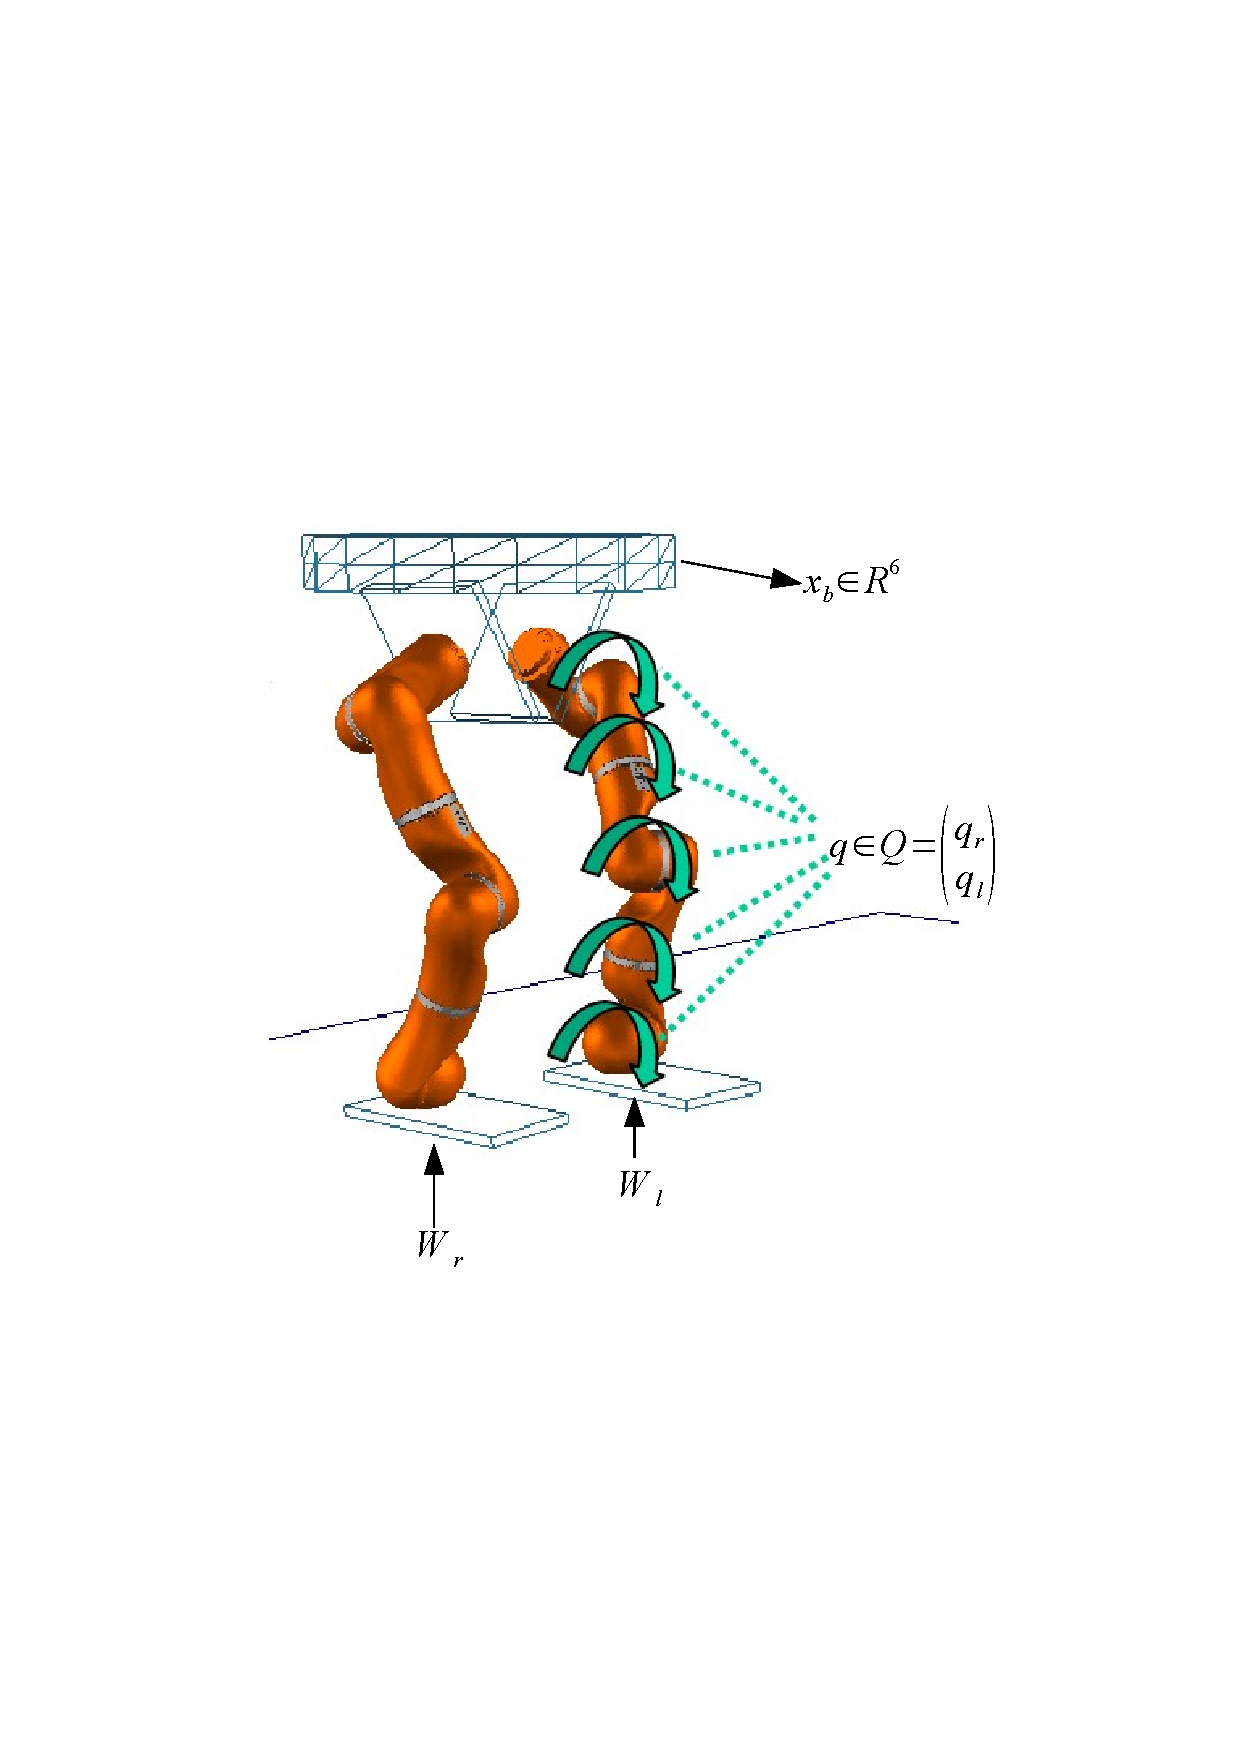
\includegraphics[trim= 10mm 80mm 10mm 80mm,scale=0.75]{Bilder/model_biped.pdf}
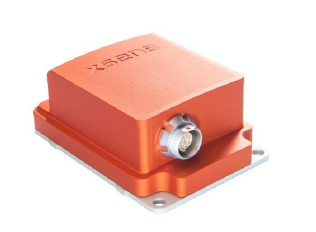
\includegraphics[scale=0.75]{Bilder/pic_imu.png}
\caption{IMU(\emph{MTi-100} mounted) on \emph{Toro}}
\label{fig:toro_imu}
\end{center}
\end{figure}
\begin{equation}
    \label{eq:imu_acc}
    a = R(a_{abs} - g)
\end{equation}
\begin{itemize}
    \item $a_{abs} $ is the absolute acceleration of the body with respect to world(spatial frame).
    \item \emph{g} is the term acceleration due to gravity $\begin{bmatrix}0 \\ 0 \\ -9.81\end{bmatrix}$.
\end{itemize}
In addition to the external accelerations, IMU also measures the acceleration due to gravity \emph{g}. The compensation for the acceleration due to gravity is given in Equation \ref{eq:imu_acc}. The measurement from the IMU is noisy. In addition to the noise there can be bias acting on the measurements. The stochastic model of the IMU is 
\begin{equation}
\label{eq:imu_noise}
\begin{split}
\tilde{a} &= a + b_a + w_a \\
\dot{b}_a &= w_{ba} \\
\tilde{\omega} &= \omega + b_\omega + w_\omega \\
\dot{b}_\omega &= w_{b\omega}
\end{split}
\end{equation}
$\tilde{a}$ is the measured acceleration from the IMU. It is composed of true acceleration \emph{a}, bias in the acceleration measurements $b_a$ and the sensor noise $w_a$. $\tilde{\omega}$ is the angular velocity measured, which comprises of true angular velocity $\omega$, bias $b_{\omega}$ and sensor noise $w_\omega$. The sensor noises $w_a$ and $w_\omega$ are modelled as zero mean Gaussian white noise. The bias in acceleration measurement is $b_a$ and that of angular velocity measurement is $b_\omega$. The bias terms are also time varying quantities but they have very slow dynamics. Bias dynamics $\dot{b}_a$ and $\dot{b}_\omega$ are modelled as first order Markov process. $w_{b\omega}$ and $w_{bf}$ are the Gaussian white noise associated with the bias. 

\section{State space representation}
The state space formulation of the dynamic model is based on Equation \ref{eq:newton_motion}. Rearranging the Equation \ref{eq:imu_noise} in terms of true acceleration and true angular velocity and substituting Equation \ref{eq:imu_acc} in \ref{eq:imu_noise} leads to state space dynamic model. 
\begin{equation}
    \label{eq:dyn_imu}
    \begin{split}
    \dot{p} &= v \\
    \dot{v} &= a = R(\tilde{a} - b_a - w_a)+g \\
    \dot{\theta} &= T^{-1}\omega = T^{-1}(\tilde{\omega} - b_\omega - w_\omega) \\
    \dot{b}_a &= w_{ba}\\
    \dot{b}_\omega &= w_{b\omega}
    \end{split}
\end{equation}
\begin{itemize}
    \item $ r = \begin{bmatrix} p_x \\ p_y \\ p_z \end{bmatrix}$ is the position of IMU measurement frame with respect to spatial frame.
    \item $ v = \begin{bmatrix} v_x \\ v_y \\ v_z \end{bmatrix} = \begin{bmatrix} \dfdx{p_x}{t} \\ \dfdx{p_y}{t} \\ \dfdx{p_z}{t} \end{bmatrix}$ is the velocity of IMU measurement frame with respect to spatial frame.
    \item $ \theta = \begin{bmatrix} \theta_x \\ \theta_y \\ \theta_z \end{bmatrix}$ is the orientation of the IMU frame with respect to spatial frame. Orientation of IMU is parametrized as RPY Euler angles. $R=R(\theta)$ is the rotation matrix that rotates a vector in body coordinate frame to spatial coordinate frame. [Appendix \ref{sec:rot_mat}].
    \item $T=T(\theta)$ is the matrix that transforms angular rate $\dot{\theta}$ to angular velocity in the body frame $\omega$ [Appendix \ref{sec:avel_trfm}].
\end{itemize}
\begin{equation}
x = \begin{bmatrix} p \\ v \\ \theta \\ b_a \\ b_{b\omega} \end{bmatrix} \in \Re^{15}
\end{equation}
\section{Prediction step}
The prediction equations of EKF are given in Equation \ref{eq:ekf_predict}. For the sake of simplicity we assume the process noise acting on the model is uncorrelated. i.e The noise acting on each state is independent $$W_k = I_n$$. $n$ is the number of states. Substituting the value of $W_k$ in Equation \ref{eq:ekf_predict}
\begin{equation}
\label{eq:imu_predict}
\begin{split}
\hat{x}_{k+1}^- &= f(\hat{x}_{k},u_{k+1},0)\\
P_{k+1}^- &= A_kP_{k}A_k^T + Q_{k}\\
\end{split}
\end{equation}
The model is discretized for the implementation of EKF. Since the time step for integration is very small $\Delta t = 1ms$ forward Euler discretization method is used to discretize the continuous time model in \ref{eq:dyn_imu}.
\begin{equation}
    \label{eq:dyn_imu_disc}
    \begin{split}
    \hat{p}_{k+1}^- &= \hat{p}_k + \Delta t \hat{v}_k + \frac{\Delta t^2}{2} \hat{R}_k (\tilde{a}_{k+1} - \hat{b}_{a,k} +g) \\
    \hat{v}_{k+1}^- &= \hat{v}_k + \Delta t \hat{R}_k (\tilde{a}_{k+1} - \hat{b}_{a,k} +g) \\
    \hat{\theta}_{k+1}^- &= \hat{\theta}_k + \Delta t \hat{T}_k^{-1}(\tilde{\omega}_{k+1} - \hat{b}_{\omega,k+1}) \\
    \hat{b}_{a,k+1}^- &= \hat{b}_{a,k}\\\
    \hat{b}_{\omega,k+1}^- &= \hat{b}_{\omega,k}
    \end{split}
\end{equation}
The system matrix is obtained by computing the Jacobian of the discretized system of equations is
\begin{equation}
    A_k = \begin{bmatrix}
    I_3 &\Delta t &\frac{\Delta t^2}{2} \dfdx{\hat{R}_k}{x}(\tilde{a}_{k+1} - \hat{b}_{a,k} +g) &-\frac{\Delta t^2}{2} \hat{R}_k &\textbf{0}_3 \\
    \textbf{0}_3 &I_3  &\Delta t \dfdx{\hat{R}_k}{x}(\tilde{a}_{k+1} - \hat{b}_{a,k} +g) &-\Delta t\hat{R}_k &\textbf{0}_3\\
    \textbf{0}_3  &\textbf{0}_3 &I_3 + \Delta t \dfdx{\hat{T}^{-1}}{x}(\tilde{\omega}_{k+1} - \hat{b}_{\omega,k+1}) &\textbf{0}_3 &\Delta t \hat{T}_k^{-1}\\
    \textbf{0}_3  &\textbf{0}_3  &\textbf{0}_3  &I_3 &\textbf{0}_3 \\
    \textbf{0}_3  &\textbf{0}_3  &\textbf{0}_3  &\textbf{0}_3 &I_3
    \end{bmatrix}
\end{equation}

\section{Update step}
The update equation of the EKF is given in Equation \ref{eq:ekf_correct}. The measurement equation of the system is given by $$\hat{y}_{k+1} = h(\hat{x}_{k+1}^-,u_{k+1},0)$$.For the sake of simplicity let us assume the measurement of noise are independent. $$V_k = I_3$$. Substituting the assumption in \ref{eq:ekf_correct}
\begin{equation}
\label{eq:imu_correct}
\begin{split}
K_{k+1} &= P_{k+1}^-\hat{C}_{k+1}^{T}(\hat{C}_{k+1}P_{k+1}^-\hat{C}_{k+1}^{T} + R_{k+1})^{-1}\\
\hat{x}_{k+1} &= \hat{x}_{k+1}^- + K_{k+1}(y_{k+1}-\hat{y}_{k+1})\\
P_{k+1} &= (I- K_{k+1}\hat{C}_{k+1})P_{k+1}^-
\end{split}
\end{equation}
The contact points are the only measurements that are considered for the update step. Figure \ref{fig:biped_feet} shows the contact points. FTS(Force torque sensor) measurement is used to compute the ZMP[Appendix \underline{Zero moment point}] of the foot and also to determine the foot that is in contact with the ground. The measurement equation is same as Equation \ref{eq:y_kin} of the multi body system model. $H_{RF} \text{ and } H_{LF} $ are formed as the composition of $H_{hip}^s H_{RF}^{hip}$ and $H_{hip}^s H_{RF}^{hip}$ respectively.
\begin{equation}
    \label{eq:imu_msr}
    \begin{split}
    y_{i,j} &= H(r,\theta) kin_j(q)p_i \hspace{2cm} \forall i=\{A,B,C,D\} \text{ and } j=\{RF,LF\} \\
    &= H_{hip}^s H_{foot}^{hip}p_i \\
    &= H p_{foot,i}^{hip}
    \end{split}
\end{equation}
\begin{itemize}
    \item $H(r,\theta)$ is the homogeneous transformation matrix of the frame attached to the IMU and the spatial frame [Appendix \ref{sec:htm}]
    \item $kin_j(q)$ computes the homogeneous transformation matrix of foot relative to hip. \emph{q} represents joint angles measured by encoders.
\end{itemize}
The measurement sensitivity matrix is computed by taking the Jacobian of the measurement equation.
\begin{equation}
        \hat{C}_{k+1} = \dfdx{\hat{y}_{k+1}}{x} = \dfdx{\hat{H}_{k+1}}{x} kin_j(q_{k+1}) p_i \hspace{1cm} \forall i=\{A,B,C,D\} \text{ and } j=\{RF,LF\} 
\end{equation}
\begin{itemize}
    \item $\dfdx{\hat{H}_{k+1}}{x}$ is the partial derivative of homogeneous transformation matrix with respect to system states. [Appendix \ref{sec:htm}]
\end{itemize}
